A set of exploratory experiments were conducted for the different proposed methods to find settings where the methods succeed at producing visually pleasing data. Due to the unstable nature of \acrshort{gans} and the limited available resources in this project, most of experiments based on \acrshort{gans} failed to do this. The few successful models also turned out to be highly sensitive to changes in network architecture, hyperparameters or training setup leaving a loot of room for improvement and further investigations. 

Of the tested methods, only the \acrshort{vae} and AEGAN was capable of producing data with some visual resemblance to the original data. The Wasserstein GAN suffered from severe mode collapse and training instability thereby resulting in only failures.

The progressive \acrshort{gan} produced promising results on the initial stages with highly downsampled data. However the proposed fade-in procedure failed, forcing the model to re-learn everything from scratch at each stage of training. At the lower stages the model was capable of recovering after the fade-in but not on the full resolution stage, similar to the normal Wasserstein \acrshort{gan}. 

To circumvent the fade-in issues of the progressive \acrshort{gan} an alternative freeze-in method of introducing the layers was tested. This approach views the introduction of the new layers as a transfer learning problem and freezes all but the newly introduced weights for a number of iterations. The discriminator output of the progressive \acrshort{gan} during fade-in and freeze-in is illustrated in figure \ref{fig:fadeVsFreeze}. In this figure one can see that the freeze-in strategy results in less varying 


-

-


The reason the progressive GAN is not featured in these results can be seen in figure \ref{fig:fadeVsFreeze}.

A comparison between a VAE and the autoencoder part of an AEGAN is shown in figure <Referera till figur>. It is clear from this illustration that the simultaneous training of the GAN caused the autoencoder to generate more visually pleasing samples.

Quantitative results can be seen in table \ref{tab:quantitative_results}.

\begin{figure}[t]
    \centering
    \begin{subfigure}[b]{0.49\textwidth}
        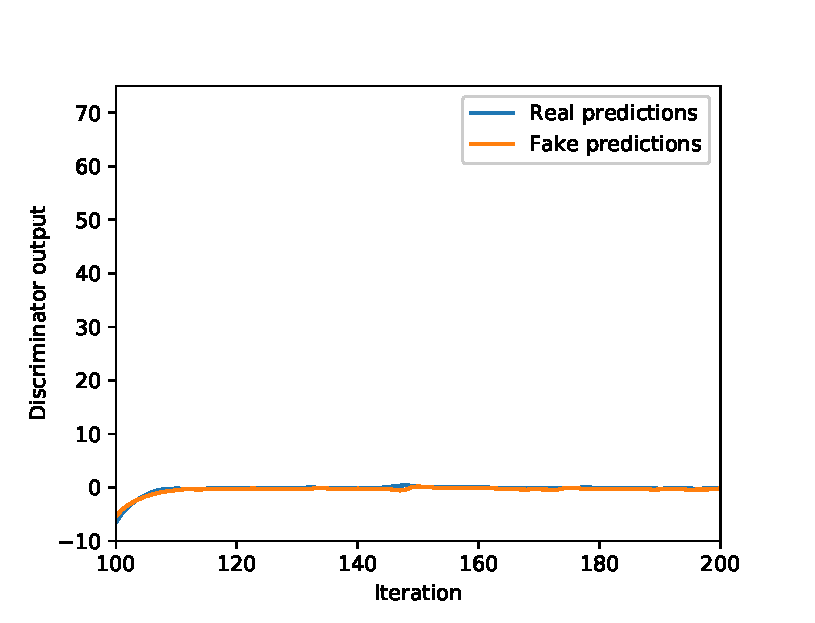
\includegraphics[width=\textwidth]{results/freezeInDG1_2.eps}
        \caption{Weight freezing in old layers}
        \label{fig:freezeInDG1}
    \end{subfigure}
    \begin{subfigure}[b]{0.49\textwidth}
        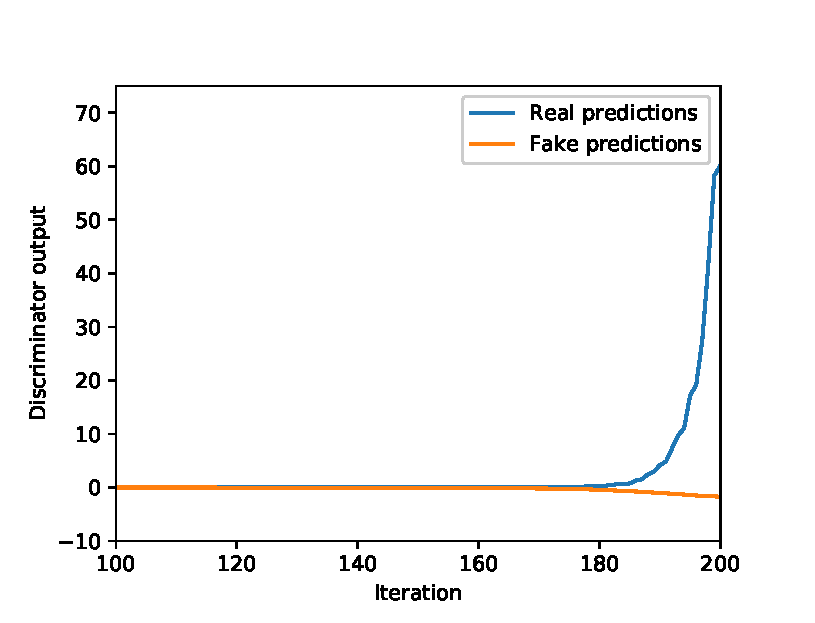
\includegraphics[width=\textwidth]{results/fadeInDG1_2.eps}
        \caption{Fade in new layers}
        \label{fig:freezeInDG2}
    \end{subfigure}
    \caption{Discriminator output on real and fake images during transition between 16x16 and 32x32 resolution images for the different transition strategies on the synthetic data se.}
    \label{fig:fadeVsFreeze}
\end{figure}

\begin{figure}[t]
    \centering
    \begin{subfigure}[b]{\textwidth}
        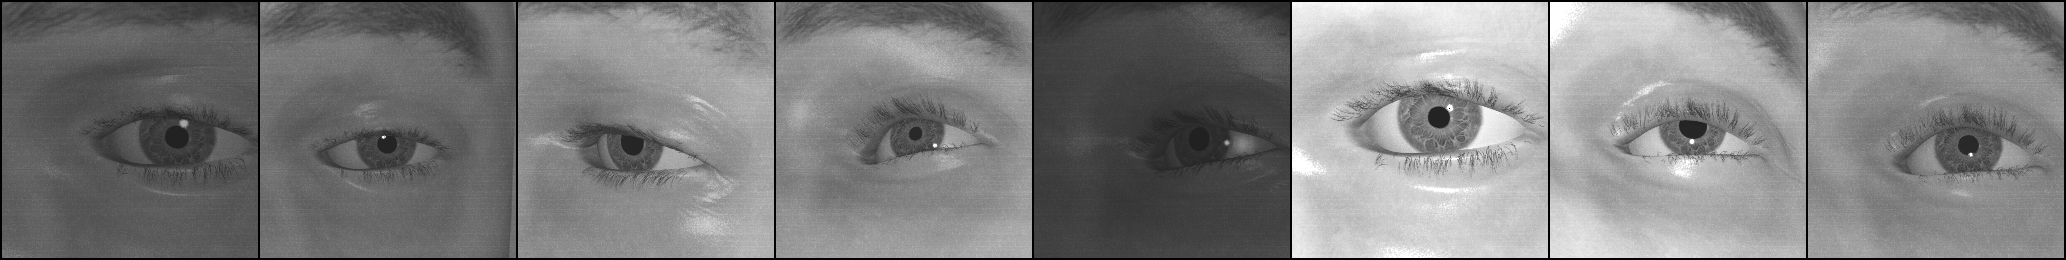
\includegraphics[width=\textwidth]{autoencoded/original.png}
        \caption{Original images}
        \label{fig:stuff}
    \end{subfigure}
    \begin{subfigure}[b]{\textwidth}
        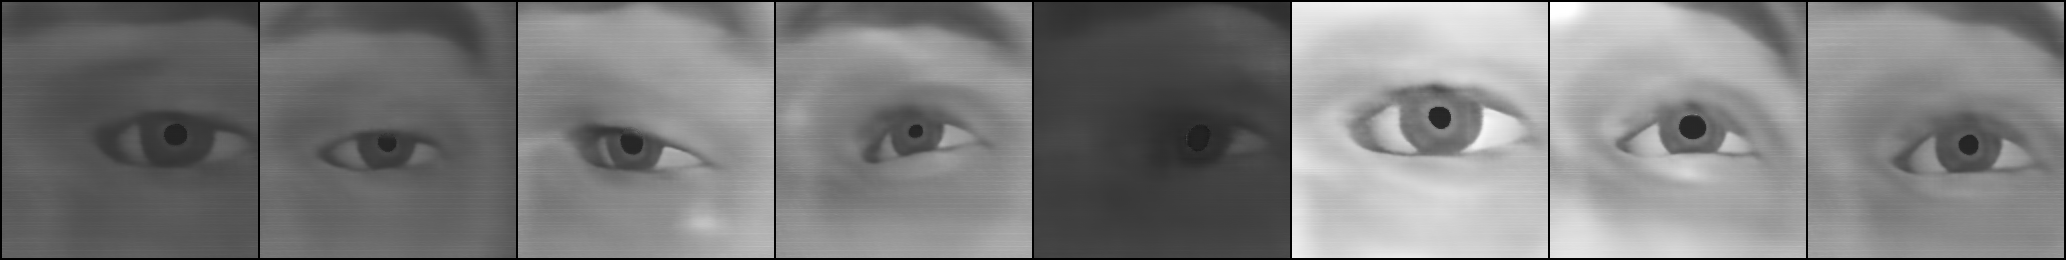
\includegraphics[width=\textwidth]{autoencoded/scaled_VAE_decoded.png}
        \caption{Decoded with VAE}
        \label{fig:stuff}
    \end{subfigure}
    \begin{subfigure}[b]{\textwidth}
        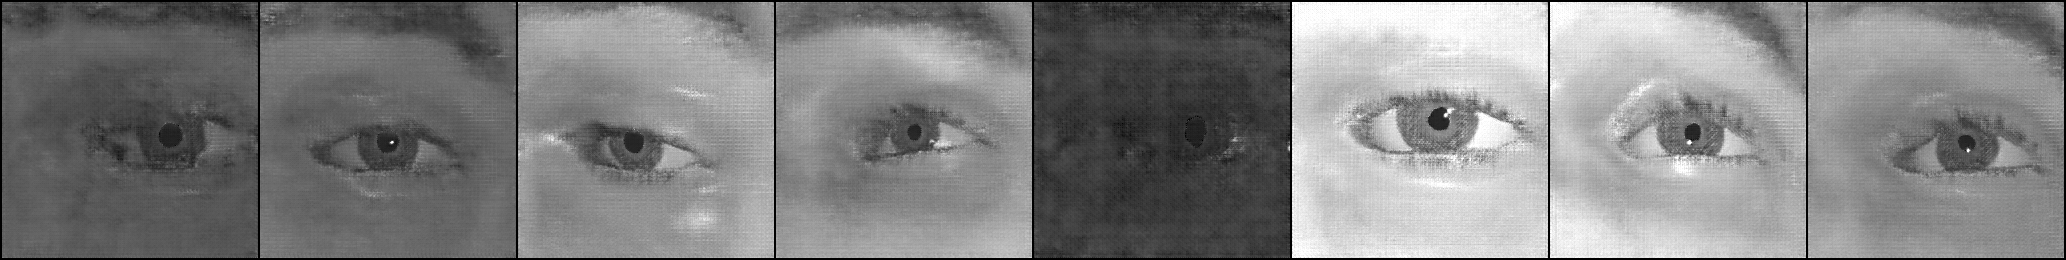
\includegraphics[width=\textwidth]{autoencoded/aegan_decoded.png}
        \caption{Decoded with AEGAN}
        \label{fig:stuff}
    \end{subfigure}
    \caption{Lorem ipsum dalar set amet ...}
    \label{fig:autoencoders}
\end{figure}

\begin{table}[t]
    \centering
    \caption{Jaccard distance between pupil regressor output and annotations for different sources of training data using synthesized data as the original data source. The JD-external measure is defined as the jaccard distance on the original test data when trained on the specified data source. The JD-internal measure is the jaccard distance on a generated test set from the same data source. The JD-incoming is for the model trained on the original data and tested on the aforementioned test set. TODO better names for this, adn write a paragraph on this}
    \label{tab:quantitative_results}
    \begin{tabular}{|l|l|l|l|l|}
        \cline{2-5}
        \multicolumn{1}{c}{ } & \multicolumn{2}{|c|}{Only generated data} & \multicolumn{2}{c|}{With original data} \\ \hline
        \textbf{Generative model} & VAE & AEGAN & VAE & AEGAN \\ \hline
        \textbf{JD-external} & 234 & 1234 & 1234 & 3454 \\
        \textbf{JD-internal} & 234 & 1234 & 1234 & 3454 \\ 
        \textbf{JD-incoming} & 234 & 1234 & 1234 & 3454 \\ \hline
    \end{tabular}
\end{table}

\begin{table}[t]
    \centering
    \caption{Jaccard distance between pupil regressor output and annotations for different sources of training data using models trained on real data as original data.}
    \label{tab:quantitative_results}
    \begin{tabular}{|l|l|l|l|l|}
        \cline{2-5}
        \multicolumn{1}{c}{ } & \multicolumn{2}{|c|}{Only generated data} & \multicolumn{2}{c|}{With original data} \\ \hline
        \textbf{Generative model} & VAE & AEGAN & VAE & AEGAN \\ \hline
        \textbf{JD-external} & 234 & 1234 & 1234 & 3454 \\
        \textbf{JD-internal} & 234 & 1234 & 1234 & 3454 \\ 
        \textbf{JD-incoming} & 234 & 1234 & 1234 & 3454 \\ \hline
    \end{tabular}
\end{table}

\begin{table}[t]
    \centering
    \caption{Jaccard distance between pupil regressor output and annotations on synthetic data}
    \label{tab:quantitative_results}
    \begin{tabular}{l|l|l}
    \hline
    %\multicolumn{3}{c}{Generator}           \\ 
    Training data type      & MEE synthetic data  & MEE Accuracy real data \\ \hline
    Original data           & $\sim$ 0.3 & 1.1     \\
    VAE                     & $\sim$ 1.7 & 1.9     \\
    VAE + original data     & 0.3 (guess) & 134     \\
    %PGAN                    & 5.4 (pessimistic guess) & 134     \\
    %PGAN + original data    & 0.3 (optimistic guess) & 134     \\
    AEGAN                   & 0.3 (optimistic guess) & 134     \\
    AEGAN + original data   & 0.3 (guess) & 134     \\
    \end{tabular}
\end{table}



%\begin{table}[t]
%    \centering
%    \caption{Number of iterations of training for the different algorithms}
%    \label{tab:quantitative_results}
%    \begin{tabular}{l|l|l}
%    \hline
%    %\multicolumn{3}{c}{Generator}           \\ 
%    Training data type      & Synthetic data  & Real data \\ \hline
%    VAE                     & 560000 & 560000 \\
%    PGAN                    & idk & idk     \\
%    AEGAN                   & 520000 & 840000   \\
%    \end{tabular}
%\end{table}

TODO: Visa kapacitet/overfitting på samma dataset, visa att genererad data är konsistent och har bra annoteringar!

<<Lägg till ett par histogram här.>>

<<Figur med referensbatch och decoded för VAE, AE och AEGAN. Inkludera L1-fel för samtliga rekonstruktioner>>


